\documentclass[conference]{IEEEtran}
\IEEEoverridecommandlockouts

% ====== Essential Packages ======
\usepackage{amsmath,amssymb,amsthm}
\usepackage{graphicx}
\usepackage{hyperref}
\usepackage{listings}
\usepackage{algorithm}
\usepackage{algpseudocode}
\usepackage{multirow}
\usepackage{booktabs}
\usepackage{caption,subcaption}
\usepackage{microtype}
\usepackage{xcolor}
\usepackage{array}
\usepackage{float}
\usepackage{enumitem}
\usepackage{authblk}
\usepackage{lipsum}

\hypersetup{
    colorlinks=true,
    allcolors=blue,
    pdftitle={Fair BC via MGDA in a 2D Battle Royale},
    pdfauthor={Kasra Fouladi},
}

% ====== Custom Commands ======
\newcommand{\R}{\mathbb{R}}
\newcommand{\E}{\mathbb{E}}
\newcommand{\Loss}{\mathcal{L}}
\newcommand{\Var}{\mathrm{Var}}
\newcommand{\Cov}{\mathrm{Cov}}

\newtheorem{theorem}{Theorem}
\newtheorem{lemma}{Lemma}
\newtheorem{proposition}{Proposition}
\newtheorem{corollary}{Corollary}
\newtheorem{remark}{Remark}

% ====== Title & Authors ======
\title{Fair BC via MGDA in a 2D Battle Royale}

\author{Kasra Fouladi\thanks{Corresponding author: \texttt{k4sr405@gmail.com}. B.Sc. student, Department of Computer Science, Iran University of Science and Technology.}}
\affil{\textbf{GitHub}: \url{https://github.com/bistoyek21-ric/StrikeForce}}

% ====== DOCUMENT START ======
\begin{document}

\maketitle

\begin{center}
\small\textit{Note: AI writing assistance was utilized for improved readability while preserving all technical integrity.}
\end{center}

\begin{abstract}
Behavioral cloning (BC) from human demonstrations often overlooks rare but critical actions due to class imbalance. We show that scalarized loss variants (inverse weighting, focal loss) fail to resolve gradient conflicts between action types. We propose BC-MGDA, which partitions the action space into semantic groups, averages the loss within each group, and applies the Multiple-Gradient Descent Algorithm to find an update direction that simultaneously improves all groups. We prove that group averaging reduces gradient variance and increases the chance of obtaining a common descent direction. We categorize five BC methods into scalarized-loss and partitioned-gradient families and design a comparison on StrikeForce, a 2D battle‑royale environment built for fair imitation learning on consumer CPUs (31x31x32 observations, 9 actions, naturally long‑tailed). StrikeForce and our baseline agents are publicly released as a reproducible benchmark. Full empirical results will be reported in the final paper.
\end{abstract}

\begin{IEEEkeywords}
behavioral cloning, multi-objective optimization, MGDA, battle royale, fairness in imitation learning, imitation learning
\end{IEEEkeywords}

\section{Introduction}
Imitation learning (IL) allows autonomous agents to learn complex behaviors from human demonstrations. Behavioral Cloning (BC), the simplest IL technique, directly maximizes the likelihood of observed actions and is widely used due to its simplicity and stability. However, BC critically suffers from \emph{action imbalance}: in many realistic tasks, especially games, the demonstrated actions follow a long‑tailed distribution. Frequent actions such as moving dominate the dataset, while rare but essential actions—shooting, healing, using items—appear far less often. Standard BC, which minimizes the average negative log‑likelihood over all frames, overfits to the majority classes and neglects the minority ones, producing policies that lack diversity and fail in situations where the rare actions are most needed.

To counteract this, practitioners often resort to scalarized loss modifications, e.g., inverse frequency weighting (BC‑IW), focal loss~\cite{lin2017focal}, or the class‑balanced loss~\cite{cui2019class}. % NEW CITATION
These methods re‑weight individual frames to emphasize rare classes, but they collapse the entire batch into a single scalar loss. Consequently, they cannot capture \emph{gradient conflicts} between action types: improving the model’s ability to shoot may require features that impair its movement, and a single scalar loss cannot explicitly resolve such trade‑offs. As a result, even after re‑weighting, the policy may still sacrifice some action types for others.

A fundamentally different approach is to treat each action type as a separate objective and seek a parameter update that improves all of them simultaneously. In multi‑task learning, the Multiple‑Gradient Descent Algorithm (MGDA)~\cite{desideri2012multiple,sener2018multi} finds a convex combination of task gradients that yields a common descent direction, guaranteeing a decrease for every task when such a direction exists. However, applying MGDA directly to per‑frame losses would involve thousands of objectives, making the problem intractable and the resulting direction noisy.

We propose \textbf{BC‑MGDA}, a method that bridges this gap. We first partition the nine core actions of our environment into three semantic groups: movement/no‑op, turning, and combat. For each training mini‑batch, we compute the average loss within each group, obtaining exactly three loss values. We then solve the MGDA quadratic program on the corresponding group gradients. This design achieves two important properties:
\begin{itemize}
    \item \textbf{Noise reduction}: Averaging frames within a group significantly reduces the variance of the gradient estimates, making the MGDA solution more reliable.
    \item \textbf{Conflict resolution}: By operating on a low‑dimensional (3‑objective) space, MGDA can explicitly balance conflicting gradient directions and, when a common descent direction exists, guarantee that all group losses decrease simultaneously.
\end{itemize}
Thus, BC‑MGDA provides a principled way to obtain \emph{Pareto‑improving} updates for all action types.

We systematically compare BC‑MGDA against four representative BC variants: standard BC, BC‑IW, BC‑Focal, and BC‑PCGrad (a partitioned method that uses gradient projection). We categorize these methods into two families: \emph{scalarized‑loss} approaches that compute a single scalar loss, and \emph{partitioned‑gradient} approaches that separate gradients by action group before combining them. Our study is conducted on \textbf{StrikeForce}, a custom 2D battle‑royale environment purpose‑built for research on fair imitation learning. StrikeForce provides a $31\times31\times32$ tensor observation, nine core actions, and a naturally long‑tailed action distribution. Crucially, the entire system—environment, agent, and training loop—runs on a consumer CPU with at most 8\,GB of RAM.

We deliberately impose this hardware constraint to make a methodological point: in a resource‑limited setting, one cannot compensate for poor algorithmic design by simply scaling up model size or training data. The architecture and training protocol must be inherently efficient and fair. Our work therefore contributes not only a new method but also a benchmark that highlights the importance of training‑protocol design under practical constraints. We publicly release the StrikeForce environment, our dataset of 256 human‑played games, and all baseline agents. Additionally, we announce a \emph{StrikeForce AI Challenge} to encourage the community to develop the strongest agent that remains playable on a PC with 8\,GB RAM and CPU only.

Our contributions are:
\begin{enumerate}
    \item A taxonomy of BC variants into scalarized‑loss and partitioned‑gradient families.
    \item BC‑MGDA, a fair BC method that uses group‑wise averaging and MGDA to obtain Pareto‑improving updates.
    \item A theoretical analysis showing that group averaging reduces gradient noise and increases MGDA feasibility.
    \item The public release of StrikeForce as a resource‑efficient benchmark for imbalanced imitation learning.
\end{enumerate}

\section{Related Work}
\subsection{Behavioral Cloning and Imbalanced Data}
Behavioral Cloning is known to suffer from compounding errors and distributional shift~\cite{ross2011reduction}. When the demonstration data is imbalanced, the policy often collapses to the majority classes. Classical remedies include inverse frequency weighting, resampling, focal loss~\cite{lin2017focal}, and the class‑balanced loss~\cite{cui2019class}. % NEW CITATION
These methods apply static, per‑frame weights to counter class imbalance. However, because they optimize a single scalar loss, they cannot explicitly resolve gradient conflicts between different action types. Recent work has explored curriculum learning and adaptive weighting, but the fundamental limitation remains: scalar losses obscure the multi‑objective nature of imitating diverse behaviors.

\subsection{Multi‑Objective Optimization and Gradient Surgery}
In multi‑task learning, gradient conflicts are common when different tasks pull the shared parameters in opposing directions. PCGrad~\cite{yu2020gradient} projects conflicting gradients onto each other’s normal plane, reducing destructive interference. CAGrad~\cite{liu2021conflict} adds a constraint to ensure a minimum per‑task improvement. MGDA~\cite{desideri2012multiple,sener2018multi} solves a quadratic program to find a convex combination of the task gradients that is a descent direction for all tasks simultaneously. Another line of work, Pareto MTL~\cite{lin2019pareto}, decomposes the problem into finding a point on the Pareto front via a different geometric approach. % NEW CITATION
When a non‑zero solution exists, every task loss is guaranteed to decrease. MGDA has been applied to multi‑modal imitation learning~\cite{peng2019multi}, where each demonstration source is treated as a separate task, but not to the problem of per‑action fairness within a single dataset. Our work is the first, to our knowledge, to use MGDA for balancing action types in behavioral cloning.

\subsection{Lightweight and Accessible Game Environments}
Many research environments for imitation learning and multi‑agent systems are computationally intensive. Neural MMO~\cite{suarez2019neural} and large‑scale battle royale simulators require GPU acceleration and substantial memory. On the other end of the spectrum, lightweight environments such as MinAtar~\cite{young2019minatar} and Griddly~\cite{bamford2020griddly} provide efficient baselines for RL, but they lack the tactical depth and observation richness needed to study fair IL with many action categories. % NEW CITATIONS
StrikeForce fills this gap: it offers a 2D top‑down battle‑royale experience with partial observability, diverse item usage, and strategic decision‑making, while running entirely on a CPU with under 100\,MB of RAM in idle mode. This makes it possible to run dozens of training runs on a single laptop, enabling thorough ablation studies and democratizing access to fair IL research. By deliberately constraining the hardware budget (8\,GB RAM, CPU only), we emphasize the efficiency of the training protocol itself, rather than relying on brute‑force scaling.

\subsection{Evaluation of Fair Imitation Learning}
Prior work on fair IL has largely focused on learning from heterogeneous demonstrators or avoiding dangerous states. In contrast, we define fairness with respect to \emph{action types}: an agent should not sacrifice any action category. Our evaluation protocol combines standard offline metrics (per‑action accuracy, macro accuracy) with in‑game performance and behavioral coverage, providing a comprehensive picture of how well each method preserves diverse skills.

\section{Preliminaries and Problem Statement}
We consider discrete-time imitation learning from a dataset $\mathcal{D} = \{(o_t, a_t)\}_{t=1}^N$, where $o_t \in \mathbb{R}^{31\times31\times32}$ are observations and $a_t \in \mathcal{A}$ are actions with $|\mathcal{A}| = 9$. The policy $\pi_\theta(a|o)$ is a neural network with parameters $\theta$, trained to minimize the standard behavioural cloning loss with an entropy regularizer:
\begin{equation}
L_{\text{BC}}(\theta) = -\frac{1}{N}\sum_{t=1}^N \log \pi_\theta(a_t|o_t) - \beta H(\pi_\theta(\cdot|o_t)),
\label{eq:bc}
\end{equation}
where $H$ is the entropy of the policy and $\beta = 0.05$.

When the action distribution in $\mathcal{D}$ is highly skewed, the single scalar loss~\eqref{eq:bc} focuses optimization on frequent actions at the expense of rare ones. To address this, we seek a learning rule that \emph{improves all action types simultaneously}. Concretely, we partition $\mathcal{A}$ into $K$ disjoint groups $G_1,\dots,G_K$ ($K=3$ in our work) and define the per-group loss as the conditional expectation
\begin{equation}
\mathcal{L}_k(\theta) = \mathbb{E}_{(o,a)\sim\mathcal{D}}\big[-\log \pi_\theta(a|o) \mid a \in G_k\big].
\label{eq:group}
\end{equation}
Let $g_k = \nabla_\theta \mathcal{L}_k(\theta)$ be the gradient of the $k$-th group loss. Our goal is to find an update direction $d$ such that
\[
\langle g_k, d \rangle < 0 \quad \text{for all } k,
\]
i.e., a \emph{Pareto-improving} direction. Such a direction exists if and only if the origin is not contained in the convex hull of the group gradients. This geometric condition directly motivates the Multiple-Gradient Descent Algorithm~\cite{desideri2012multiple}, which solves a small quadratic program to find the best common descent direction. In practice, the true gradients $g_k$ are replaced by their mini-batch estimates as described in Section~\ref{sec:methodology}.

\section{The StrikeForce Environment}
StrikeForce is a 2D top-down survival shooter written in C++ using SFML and LibTorch. It features:
\begin{itemize}
    \item \textbf{Map}: three floors, each $30\times100$ tiles, with walls, portals, chests, and destructible blocks.
    \item \textbf{Observation}: a $31\times31$ local grid centered on the agent, with 32 semantic channels (entities, health, items, bullets, etc.).
    \item \textbf{Action space}: 9 core actions---no-op, turn left/right, move in four directions, punch, shoot.
    \item \textbf{Game modes}: Solo (zombie waves), Timer, Squad (5v5), Battle Royale (online multiplayer), and AI Battle Royale (spectator).
    \item \textbf{Logging}: frame-by-frame recording of the observation tensor and action for IL datasets.
\end{itemize}
The environment is fully deterministic and controlled by a master seed. Thanks to this property, an entire episode can be reconstructed exactly from only the initial seed and the sequence of actions. Consequently, IL datasets do not need to store the high-dimensional observation tensors; it suffices to save the seed and the action list, reducing the storage footprint from tens of megabytes per episode to less than a kilobyte. For convenience, the built-in logger can output either the complete observation stream or the compact seed-action representation.

Human demonstrations in StrikeForce exhibit a naturally long-tailed action distribution, with movement actions dominating and combat actions appearing rarely. This imbalance makes the environment an ideal testbed for studying fairness in behavioural cloning.

\begin{figure}[H]
  \centering
  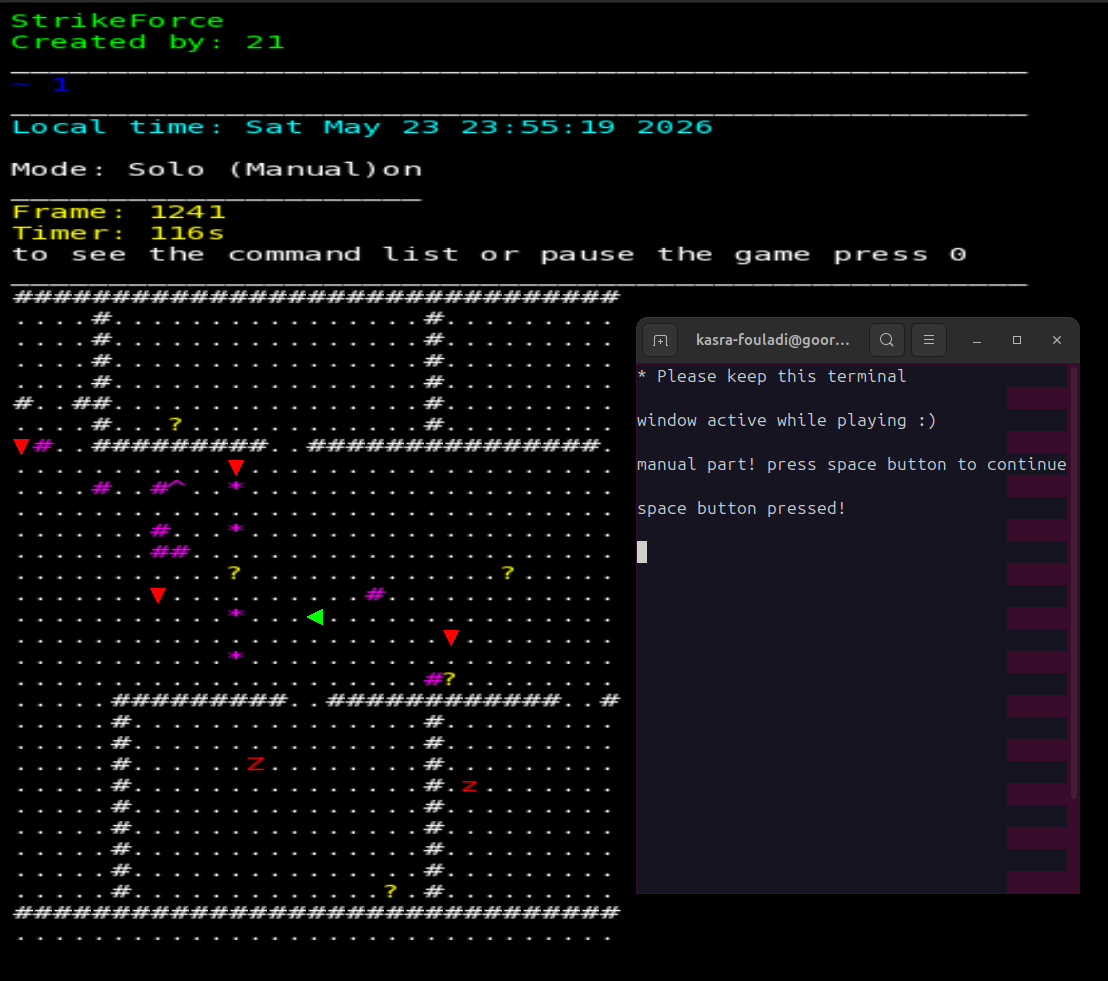
\includegraphics[width=0.7\linewidth]{figs/strikeforce-screenshot.png}
  \caption{Screenshot from StrikeForce. The agent (green triangle) perceives a $31\times31$ grid.}
  \label{fig:screenshot}
\end{figure}

\section{Methodology}
\label{sec:methodology}
All compared methods use the same network architecture: a GameCNN encoder (4 strided convolutional layers) followed by two GRU cells and residual policy/value heads. The difference lies solely in how the loss is constructed and how gradients are combined.

\subsection{Network Architecture}
\begin{figure}[H]
  \centering
  \includegraphics[width=\linewidth]{figs/architecture.png}
  \caption{Shared architecture: GameCNN $\to$ GRU layers $\to$ policy/value heads. The value head is unused during BC training but kept for compatibility with future RL extensions.}
  \label{fig:arch}
\end{figure}
The GameCNN processes the $31\times31\times32$ input through four $3\times3$ convolutions with stride 2, producing a feature vector that is normalized by its L1 norm. A two-layer GRU captures temporal dependencies. The policy head (ResBlock + linear) outputs a softmax over 9 actions; the value head outputs a scalar.

\subsection{Scalarized Loss Methods}
These methods compute a single scalar loss from the batch and perform one backward pass.

\subsubsection{Standard BC}
Loss defined in (\ref{eq:bc}). No special treatment of rare actions.

\subsubsection{BC-IW (Inverse Frequency Weighting)}
Each frame is weighted by $w_a = 1/(p_a + \epsilon)$, where $p_a$ is the global frequency of action $a$. This up-weights rare actions but is static and cannot handle dynamic conflicts. Even advanced static weighting schemes such as the class‑balanced loss~\cite{cui2019class} share the same fundamental limitation. % NEW CITATION USAGE

\subsubsection{BC-Focal (Focal Loss)}
Focal loss~\cite{lin2017focal} reduces the weight for well-classified examples: $w_t = (1-\pi_\theta(a_t|o_t))^\gamma$, with $\gamma=2$. It focuses on hard frames but still uses a single scalar loss.

\subsection{Partitioned Gradient Methods}
We partition the 9 actions into $K=3$ groups according to their semantics:
\begin{align*}
G_1 &= \{\text{no-op, move up, move left, move down, move right}\},\\
G_2 &= \{\text{turn clockwise, turn counter-clockwise}\},\\
G_3 &= \{\text{punch, shoot}\}.
\end{align*}
For a given batch $B$, let $B_k \subseteq B$ be the subset of frames whose action belongs to $G_k$.
Define the per-group loss as
\begin{equation}
L_k(\theta) = -\frac{1}{|B_k|}\sum_{t \in B_k} \log \pi_\theta(a_t|o_t),
\label{eq:group_loss}
\end{equation}
with the convention that $L_k = 0$ and its gradient $g_k = 0$ if $B_k = \emptyset$.
We then compute the gradient of each group, $g_k = \nabla_\theta L_k$, and combine them according to one of the strategies below.

\subsubsection{BC-PCGrad}
When two group gradients have a negative inner product, following one gradient may increase the other group's loss. PCGrad~\cite{yu2020gradient} addresses this by projecting each conflicting gradient onto the normal plane of the other: for every pair $(g_i,g_j)$ with $g_i\!\cdot\!g_j < 0$, it computes $g_i' = g_i - \frac{g_i\cdot g_j}{\|g_j\|^2}g_j$ and similarly for $g_j$. This removes the mutually harmful components while preserving the rest of the gradient signal. The final update direction is the average of all (possibly projected) $g_k$. Although PCGrad reduces destructive interference, it does not guarantee that the resulting direction strictly improves all groups, unlike MGDA.

\subsubsection{BC-MGDA (Ours)}
BC-MGDA explicitly finds a convex combination of the group gradients with minimal norm:
\begin{equation}
\alpha^* = \text{ArgMin}_{\alpha\ge 0,\;\sum_{k=1}^K \alpha_k = 1} \Bigl\|\sum_{k=1}^K \alpha_k g_k\Bigr\|^2.
\label{eq:mgda}
\end{equation}
If the optimal value is strictly positive, the direction $d = -\sum_k \alpha_k^* g_k$ satisfies $\langle g_k, d\rangle < 0$ for every $k$, guaranteeing that each $L_k$ decreases locally~\cite{desideri2012multiple}. If the minimum is zero (a Pareto-stationary point), we fall back to equal weights $\alpha_k = 1/K$, which recovers the standard BC update direction and ensures at least the unweighted sum of losses decreases.

\subsection{Implementation Details}
The quadratic program \eqref{eq:mgda} has only $K=3$ variables; we solve it exactly by enumerating all non-empty subsets of groups (active-set search over $2^3-1 = 7$ possibilities). The per-group gradients $g_k$ are obtained by performing $K$ separate forward-backward passes (one per group), i.e., without retaining the computation graph. This avoids the $K$-fold memory increase of the graph and keeps the memory footprint identical to standard BC (see Section~\ref{sec:complexity} for a detailed complexity analysis). We use the AdamW optimizer with a learning rate of $3\times10^{-4}$ and a batch size $B=16$. The network has approximately 1.2 million trainable parameters.

\section{Theoretical Analysis}

\subsection{Variance Reduction via Group Averaging}
For each action group $k$, the loss $L_k$ is the average of $N_k$ per-frame losses.
Let $\sigma^2$ be the variance of the gradient of a single frame (assumed bounded).
Then
\[
\Var(g_k) = \frac{\sigma^2}{N_k}.
\]
Thus, grouping directly reduces the gradient noise by a factor of $N_k$, making the per-group direction estimates more reliable.

\subsection{Compatibility and Finite‑Sample Guarantee}
Let $\bar{g}_k = \nabla \mathcal{L}_k(\theta)$ be the true (population) gradients, and
$g_k = \bar{g}_k + \epsilon_k$ their empirical estimates from a batch, with $\E[\epsilon_k]=0$ and
$\Var(\epsilon_k) = \mathcal{O}(1/N_k)$.
We say the true gradients are \emph{compatible} if
$\min_{\alpha\ge 0,\sum\alpha_k=1} \|\sum_k \alpha_k \bar{g}_k\|^2 > 0$,
i.e., the origin is outside the convex hull of $\{\bar{g}_k\}$.

\begin{proposition}[Convergence of empirical compatibility]
\label{prop:compat}
Assume $\|\epsilon_k\|$ is sub-Gaussian with variance proxy $\tau^2/N_k$.
If the true gradients are compatible, then for any $\delta\in(0,1)$ there exists a constant $C>0$ such that
when all $N_k \ge C\tau^2 \log(K/\delta)$,
\[
\Pr\left( \min_{\alpha\ge 0,\sum\alpha_k=1} \big\|\sum_k \alpha_k g_k\big\|^2 > 0 \right) \ge 1-\delta.
\]
\end{proposition}
\begin{proof}
The convex hull of $\{g_k\}$ is within the Minkowski sum of the convex hull of $\{\bar{g}_k\}$ and a ball of radius $\max_k\|\epsilon_k\|$.
Since the origin is outside the true hull by a positive margin $\Delta>0$, it remains outside the empirical hull as long as
$\max_k\|\epsilon_k\| < \Delta/2$.
By a union bound over the $K$ groups and sub-Gaussian tail bounds,
$\Pr(\max_k\|\epsilon_k\| \ge t) \le \sum_k 2\exp(-t^2 N_k/(2\tau^2))$.
Choosing $t=\Delta/2$ and $N_k$ sufficiently large gives the claimed probability.
\end{proof}

Proposition~\ref{prop:compat} explains why group averaging and large batch sizes for each group increase the chance of MGDA producing a strict descent direction instead of falling back to equal weights.

\subsection{Pareto Stationarity and Fairness}
When the MGDA objective \eqref{eq:mgda} attains zero, the resulting convex coefficients satisfy
$\sum_k \alpha_k^* g_k = 0,\ \alpha_k^*\ge 0,\ \sum_k \alpha_k^*=1$.
This is exactly the first-order necessary condition for a \emph{Pareto-stationary} point~\cite{desideri2012multiple},
meaning no local direction can improve all objectives simultaneously.

Conversely, when the minimum is positive, the direction $d = -\sum_k \alpha_k^* g_k$ satisfies
$\langle g_k, d\rangle < 0$ for every $k$, guaranteeing a strict reduction in each $\mathcal{L}_k$.

\begin{proposition}[Expected Pareto improvement]
\label{prop:improve}
Assume each $\mathcal{L}_k$ is $L$-smooth and the gradient estimates are unbiased.
If the empirical MGDA solution gives a direction $d$ and a constant $\epsilon>0$ such that
$\langle g_k, d\rangle \le -\epsilon$ for all $k$, then for a sufficiently small step size $\eta$,
\[
\E[\mathcal{L}_k(\theta_{t+1})] \le \mathcal{L}_k(\theta_t) - \eta\epsilon + O(\eta^2 L).
\]
\end{proposition}
\begin{proof}
By $L$-smoothness,
$\mathcal{L}_k(\theta_{t+1}) \le \mathcal{L}_k(\theta_t) + \eta \langle \nabla\mathcal{L}_k(\theta_t), d\rangle + \frac{L}{2}\eta^2 \|d\|^2$.
Taking expectations and noting $\E[\langle \nabla\mathcal{L}_k, d\rangle] = \langle \E[\nabla\mathcal{L}_k], d\rangle = \langle \bar{g}_k, d\rangle$,
while $\langle \bar{g}_k, d\rangle = \langle g_k, d\rangle - \langle \epsilon_k, d\rangle$.
From the assumption $\langle g_k, d\rangle \le -\epsilon$ and $\E[\epsilon_k]=0$, we obtain the result.
\end{proof}

Proposition~\ref{prop:improve} formalises the guarantee that each group’s loss decreases in expectation,
as long as the empirical gradients indicate a common descent direction.

\subsection{Computational Complexity}
\label{sec:complexity}
We analyse two strategies for obtaining the per-group gradients $g_k$ in the MGDA step:
\textit{(a) retain graph}: compute a single forward pass and perform $K$ backward passes on the retained computational graph,
\textit{(b) recompute}: run $K$ separate forward passes, each immediately followed by its own backward pass.
For classic BC there is one forward and one backward.

Let $F$ and $B$ denote the time for one forward and one backward pass, respectively.
Let $M_{\text{act}}$ be the peak memory used for activations (forward state),
and $M_{\text{graph}}$ the memory needed to store the computation graph for one backward pass.
In typical reverse‑mode automatic differentiation, $B \approx 2\,F$ and $M_{\text{graph}} \approx M_{\text{act}}$.

\begin{table}[H]
\centering
\caption{Time and memory complexity of gradient computation per update.}
\begin{tabular}{lcc}
\toprule
Method & Time & Memory \\
\midrule
Classic BC                    & $O(F + B)$               & $O(M_{\text{act}} + M_{\text{graph}})$ \\
MGDA (retain graph)           & $O(F + K\cdot B)$        & $O(M_{\text{act}} + K\cdot M_{\text{graph}})$ \\
MGDA (recompute)              & $O(K\cdot(F + B))$       & $O(M_{\text{act}} + M_{\text{graph}})$ \\
\bottomrule
\end{tabular}
\label{tab:complexity}
\end{table}

Table~\ref{tab:complexity} shows the trade‑off: retaining the graph saves $K-1$ forward passes at the cost of a $K$‑fold increase in graph memory.
Because $K=3$ in our setup, both strategies are feasible on a single GPU.
We adopt the \textit{recompute} strategy in our experiments, since it reuses the standard training loop and avoids the risk of out‑of‑memory errors when scaling to larger models.

\section{Experimental Design}
We now outline the planned evaluation protocol; empirical results will be added in the final manuscript.

\subsection{Dataset}
256 human-played games at difficulty level 10 (1024 consecutive frames each) are recorded, yielding $\approx262{,}000$ frames. The dataset is split 80/20 by game.

\subsection{Baselines}
The five methods described in Section \ref{sec:methodology} are compared: Standard BC, BC-IW, BC-Focal, BC-PCGrad, and BC-MGDA. All methods share the same architecture, optimizer, and hyperparameters.

\subsection{Metrics}
\begin{itemize}
    \item \textbf{Offline imitation accuracy}: per-action accuracy, group accuracy, macro accuracy (mean of three groups).
    \item \textbf{Online game performance}: success rate (50 kills), average kills, survival time, loot, chests opened (Solo level 10, 30 episodes).
    \item \textbf{Behavioral coverage}: normalized entropy of the action distribution.
    \item \textbf{Inference cost}: latency per prediction (ms) and model memory (MB) on a CPU.
    \item \textbf{Gradient conflict index}: fraction of negative-cosine group gradient pairs during training.
\end{itemize}

\subsection{Expected Trends}
We hypothesize that partitioned methods, especially BC-MGDA, will outperform scalarized methods on macro accuracy, rare-action accuracy, and in-game performance, while maintaining similar inference cost. The gradient conflict index should be lower for BC-MGDA.

\section{Conclusion and Future Work}
We have presented a systematic comparison of BC variants for action-imbalanced imitation learning, categorizing them into scalarized-loss and partitioned-gradient families. Our proposed BC-MGDA uses action-group averaging and MGDA to guarantee fair improvement across all action types. Theoretical analysis confirms that group averaging reduces gradient noise and increases MGDA feasibility. The StrikeForce environment provides a lightweight, realistic testbed for this line of research.

All code, data, and baselines are publicly available. We invite the community to participate in the \textbf{StrikeForce AI Challenge}: build the strongest agent that runs on a PC with 8\,GB RAM and CPU only.

Future work includes extending BC-MGDA to hierarchical policies, online IL (DAgger) with multi-objective updates, and distributed training to further reduce gradient noise.

\bibliographystyle{IEEEtran}
\bibliography{refs}

\end{document}